\documentclass{article}
\usepackage{listings}
\usepackage{xcolor}


\definecolor{dkgreen}{rgb}{0,0.6,0}
\definecolor{gray}{rgb}{0.5,0.5,0.5}
\definecolor{mauve}{rgb}{0.58,0,0.82}

\definecolor{eclipseStrings}{RGB}{42,0.0,255}
\definecolor{eclipseKeywords}{RGB}{127,0,85}
\colorlet{numb}{magenta!60!black}

\lstdefinelanguage{json}{
	basicstyle=\normalfont\ttfamily,
	commentstyle=\color{eclipseStrings}, % style of comment
	stringstyle=\color{eclipseKeywords}, % style of strings
	numbers=left,
	numberstyle=\scriptsize,
	stepnumber=1,
	numbersep=8pt,
	showstringspaces=false,
	breaklines=true,
	frame=lines,
	backgroundcolor=\color{gray}, %only if you like
	string=[s]{"}{"},
	comment=[l]{:\ "},
	morecomment=[l]{:"},
	literate=
	*{0}{{{\color{numb}0}}}{1}
	{1}{{{\color{numb}1}}}{1}
	{2}{{{\color{numb}2}}}{1}
	{3}{{{\color{numb}3}}}{1}
	{4}{{{\color{numb}4}}}{1}
	{5}{{{\color{numb}5}}}{1}
	{6}{{{\color{numb}6}}}{1}
	{7}{{{\color{numb}7}}}{1}
	{8}{{{\color{numb}8}}}{1}
	{9}{{{\color{numb}9}}}{1}
}
\lstset{language=SQL,
	basicstyle={\small\ttfamily},
	belowskip=3mm,
	breakatwhitespace=true,
	breaklines=true,
	classoffset=0,
	columns=flexible,
	commentstyle=\color{dkgreen},
	framexleftmargin=0.25em,
	frameshape={}{yy}{}{}, %To remove to vertical lines on left, set `frameshape={}{}{}{}`
	keywordstyle=\color{blue},
	numbers=none, %If you want line numbers, set `numbers=left`
	numberstyle=\tiny\color{gray},
	showstringspaces=false,
	stringstyle=\color{mauve},
	tabsize=3,
	xleftmargin =1em
}
\lstset{
	language=Java,
	basicstyle=\ttfamily\footnotesize,
	keywordstyle=\color{blue}\bfseries,
	stringstyle=\color{red},
	commentstyle=\color{green},
	numbers=left,
	numberstyle=\tiny,
	stepnumber=1,
	numbersep=5pt,
	showspaces=false,
	showstringspaces=false,
	showtabs=false,
	frame=single,
	tabsize=2,
	breaklines=true,
	breakatwhitespace=false,
	escapeinside={\%*}{*)}
}
\usepackage{amssymb}
\usepackage{tabularx}
\usepackage{longtable}
\usepackage[utf8]{inputenc}
\usepackage{pgfplots}
\pgfplotsset{compat=1.18}
\usepackage{pgfplotstable}
\usepackage{graphicx}
\usepackage{geometry}
\usepackage{lmodern}
\usepackage{microtype}
\usepackage{fancyhdr}
\usepackage{hyperref}
\geometry{a4paper, margin=1in}

% en-têtes/pieds de page
\pagestyle{fancy}
\fancyhead[L]{Rapport de stage - OPT-NC}
\fancyhead[R]{Morgan CARRE}
\fancyfoot[C]{\thepage}


\begin{document}
	
	\begin{titlepage}
		\begin{center}
			{\LARGE \textbf{Rapport de Stage}} \\[1.5cm]
			{\large Effectué du \textbf{09/12/2024} au \textbf{[à déterminer]}} \\[1cm]
			
			
			
			{\large Réalisé au sein de la société :} \\[1cm]
			{\Large \textbf{DSI/GLIA OPT-NC}} \\[1cm]
			
			\includegraphics[width=0.3\textwidth]{asset/logo_opt.jpg} \\[1cm] 
			
			
			\textbf{à Nouméa} \\[1cm]
			
			{\large \textbf{Développement d'une API REST des forfaits télécoms conteneurisée}} \\[1cm]
			
			{\large Présenté par :} \\[1cm]
			{\LARGE \textbf{Morgan CARRE}} \\[0.5cm]
			Étudiant en Licence Informatique, Semestre 5 \\[0.5cm]
			\textbf{Université de la Nouvelle-Calédonie} \\[0.5cm]
			
			\includegraphics[width=0.2\textwidth]{asset/logo_universite.jpg} \\[2cm]
			
			{\large Supervisé par : \textbf{Adrien SALES}} \\[0.5cm]
		\end{center}
	\end{titlepage}
	\newpage
	\begin{abstract}
		Dans le cadre de mon stage à l'Université de la Nouvelle-Calédonie (UNC), en collaboration avec l'Office des Postes et Télécommunications de Nouvelle-Calédonie (OPT-NC) supervisé par Adrien SALES, j'ai travaillé sur le développement d'une API permettant de fournir des informations sur les différents forfaits télécoms. Ce projet a pour objectif de rendre les données publiques liées aux offres mobiles plus accessibles, en utilisant des outils modernes pour assurer une solution efficace et évolutive.
		
		L'API repose sur une stack technologique composée de Quarkus pour le développement de microservices performants, Flyway pour la gestion des migrations de base de données, et une base de données H2 pour le développement et les tests. 
		
		Ce rapport détaille les méthodologies adoptées, les technologies choisies et les différentes étapes de réalisation du projet, tout en mettant en lumière les défis rencontrés.
	\end{abstract}
	\newpage
	\section*{Remerciements}
	
	Je tiens à exprimer mes remerciements à toutes les personnes qui ont contribué à la réussite de ce stage et à l’élaboration de ce rapport.
	
	Tout d’abord, je remercie \textbf{Adrien SALES}, mon maître de stage, pour son accompagnement, sa disponibilité et ses conseils précieux tout au long de ce stage. Son expertise et ses retours constructifs ont grandement enrichi mon apprentissage.
	
	Je tiens également à remercier Vinh Faucher du département \textbf{DSI/GLIA} de l’OPT-NC pour ses conseils m'ayant permis de bien débuter mon stage.
	
	Je remercie également \textbf{M. Salmon} d’avoir accepté d’être mon enseignant référent pour ce stage.
		
	% à compléter au fil du stage
	\newpage
	\tableofcontents
	%à compléter : titre et sous titres
	\newpage
	\section{Introduction}
	
	\subsection{Annonce du stage}
	
	Du \textbf{09 décembre 2024} au \textbf{[à déterminer]}, j’ai effectué un stage au sein de l’entreprise \textbf{OPT} (située à Nouméa, Nouvelle-Calédonie). Au cours de ce stage au département \textbf{DSI/GLIA (Direction des Systèmes d'Information / Génie Logiciel Inter-Applicatif)}, j’ai eu l’occasion de me plonger dans le développement d’une API permettant de fournir des informations sur les différents forfaits télécoms proposés par l’entreprise.
	
	Ce stage a été pour moi une opportunité d’explorer plusieurs aspects clés du métier de développeur \textbf{backend}, notamment en matière de gestion de bases de données, d’architecture de microservices, et de l’utilisation des technologies modernes comme Quarkus et Flyway. J’ai également pu développer des compétences techniques liées à la conception d’API REST.
	
	\subsection{Bref descriptif de l’entreprise et du déroulement du stage}
	
	L’Office des Postes et Télécommunications de Nouvelle-Calédonie (\textbf{OPT-NC}) est un acteur incontournable en Nouvelle-Calédonie, intervenant dans les domaines des télécommunications, de la finance, et des services postaux (et couvrant ainsi un large éventail de secteurs d'activité). L’entreprise propose des solutions variées allant des forfaits mobiles et connexions Internet aux services financiers et de distribution postale.
	
	Au sein de son département \textbf{DSI/GLIA}, j’ai intégré une équipe dynamique spécialisée dans le développement et la gestion de solutions logicielles.
	
	
	Supervisé par \textbf{Adrien SALES}, chef de section de l’équipe \textbf{GLIA}, j’ai bénéficié d’un encadrement rigoureux, favorisant l’apprentissage et la réalisation des différentes missions. Parmi ces missions, j’ai été chargé de concevoir une architecture basée sur Quarkus et Flyway, tout en suivant les bonnes pratiques de développement logiciel.
	
	\subsection{Problématique et objectifs du rapport}
	
	Ce stage m’a permis de contribuer au développement d’une API REST destinée à centraliser et rendre accessibles les informations sur les forfaits télécoms proposés par l’OPT-NC. L’objectif principal était de créer un outil moderne et fonctionnel, facilitant l’accès à ces données et leur utilisation dans d’éventuelles applications ou analyses.
	
	Ce rapport se concentre sur le processus de développement de l’API, en détaillant les étapes de conception, les choix technologiques réalisés, ainsi que les difficultés techniques rencontrées et les solutions mises en œuvre.
	
	\newpage
	\section{Méthodologie et outils}
	
	\subsection{Méthodologie de travail}
	
	Durant ce stage, j'ai suivi une approche de travail progressive, divisant le développement de l'API en plusieurs tâches spécifiques (appelées \textit{issues}). Chaque tâche correspondait à une fonctionnalité ou une étape précise du projet.
	
	Une fois une tâche terminée, je soumettais mon travail pour vérification à travers une demande spécifique appelée \textit{pull request}. Mon maître de stage, Adrien SALES, examinait ces propositions, identifiait d'éventuelles améliorations ou corrections, et me fournissait des retours. Après validation, les modifications étaient intégrées à la branche principale du projet, garantissant ainsi une progression structurée et contrôlée.
	
	Ce processus a été appliqué tout au long du projet pour assurer la qualité du code et une bonne gestion des étapes de développement.
	
	\subsection{Stack}
	
	Voici les principaux outils et technologies que j’ai utilisés pour ce projet :
\begin{itemize}
	\item \textbf{Ubunutu} : Système d'exploitation Linux utilisé comme environnement de développement pour le projet.
	\item \textbf{Java} : Langage de programmation principal utilisé pour le développement de l'API.
	\item \textbf{Maven} : Outil de gestion de projet et des dépendances.
	\item \textbf{Quarkus} : Framework Java pour le développement de microservices performants.
	\item \textbf{Flyway} : Outil de gestion des migrations de base de données, assurant la cohérence du schéma de données.
	\item \textbf{H2 Database} : Base de données embarquée utilisée pour les phases de développement et de test.
	\item \textbf{Git et GitHub} : Pour la gestion des versions et la collaboration.
	\item \textbf{Visual Studio Code} : Environnement de développement intégré.
	\item \textbf{HTTPie} : Outil en ligne de commande pour tester les endpoints de l'API.
	\item \textbf{Podman} : Outil pour la gestion et l'exécution de conteneurs, utilisé pour tester l'API en environnement conteneurisé.
	\item \textbf{Redocly} : Outil utilisé pour générer de la documentation statique à partir des spécifications OpenAPI.
	\item\textbf{Bump.sh} : Outil similaire à Redocly avec des fonctionnalités supplémentaires.
	\item \textbf{Jib} : Outil intégré à Maven pour créer des images conteneurisées sans utiliser de \texttt{Dockerfile}. Il simplifie la conteneurisation et génère des images légères et optimisées.
	\item \textbf{SonarQube} : Outil d'analyse de la qualité du code qui détecte les problèmes, les vulnérabilités et les redondances, améliorant ainsi la qualité et la sécurité du code.
\end{itemize}
	
	\section{Première tâche : conversion des sous-tâches en issues}
	
	La première tâche qui m’a été confiée au début de mon stage était de convertir une liste de sous-tâches fournies par mon maître de stage, Adrien SALES, en \textit{issues} distinctes sur \textbf{Github}. Cette démarche avait pour but de structurer et d’organiser les différentes étapes nécessaires à la réalisation de l’endpoint \texttt{/offres}, qui devait permettre de lister les types de forfaits, leurs pages de référence et une description associée.
	
	\subsection{Contexte}
	
	L’issue principale intitulée \textit{/offres : Lister les types d'abonnements \#1} décrivait les objectifs généraux et les actions attendues pour atteindre ce résultat. Voici les différentes sous-tâches qui devaient être transformées en issues individuelles :
	
	\begin{itemize}
		\item Étudier les données pour l'API \texttt{/offres} (\#4)
		\item intialiser le projet Quarkus (\#5)
		\item Comprendre le rôle de Flyway
		\item Implémenter l'endpoint \texttt{/offres} avec Flyway
		\item Documenter avec des spécifications OpenAPI complètes
		\item Montrer un exemple d’appel avec \texttt{httpie}
		\item Implémentation au sein de Microcks (article à venir)
		\item Builder l’image en local avec \texttt{podman}
		\item Exécuter l’image en local avec \texttt{podman} et visualisation via [Podman Desktop](https://podman-desktop.io/)
		\item Générer la documentation OpenAPI
		\item Ajouter une CI pour tester le build Maven
		\item Mettre en œuvre des tests unitaires (seuil minimal 10\%)
		\item Lire des articles et regarder des vidéos sur l’automatisation de la documentation API avec GitHub, Redocly, et OpenAPI
		\item Générer une documentation HTML statique avec Redocly
		\item Livrer une première version du rapport au format \LaTeX{} : abstract et introduction
	\end{itemize}
	
	Pour illustrer la structuration et la mise en forme des issues, voici un exemple concret d’une issue que j’ai créée dans le cadre de cette tâche. Cela permet de visualiser comment chaque sous-tâche a été documentée et organisée pour garantir un suivi efficace.
	
	\begin{center}
		\textbf{Exemple d'issue mise en forme :}
	\end{center}
	
	\vspace{0.5cm}
	\begin{center}
		\includegraphics[width=0.8\textwidth]{asset/ex_issue.png}
	\end{center}
	
	Ce format inclut le titre de l’issue, une description détaillée des objectifs, et parfois des liens vers des ressources ou des outils nécessaires à sa réalisation.
	
	J’ai donc créé une issue distincte pour chaque sous-tâche, en précisant le contexte, les objectifs et les résultats attendus. Cette structuration a permis une meilleure visibilité sur les étapes du projet, tout en facilitant le suivi et la validation des différentes phases par mon maître de stage.
	\newpage
	\section{Identification des types de forfaits et création du fichier \texttt{offres.csv}}
	
	Ma deuxième tâche a consisté à identifier les différents types de forfaits disponibles sur la page de l’OPT intitulée \textit{"Identifiez le forfait qui vous ressemble"} (voir capture d’écran ci-dessous). Pour cela, j’ai analysé les caractéristiques propres à chaque forfait, notamment leur nom, leur description et leur utilisation, afin de les préparer sous une forme exploitable.
	
	\begin{figure}[h!]
		\centering
		\includegraphics[width=0.8\textwidth]{asset/page_forfait.png}
		\caption{Page \textit{"Identifiez le forfait qui vous ressemble"} sur le site de l’OPT.}
		\label{fig:page_forfait}
	\end{figure}
	
	Après cette analyse, j’ai structuré ces informations dans un fichier au format \texttt{CSV}, nommé \texttt{offres.csv}. Ce fichier contient les champs suivants : l’identifiant (\texttt{id}), le nom (\texttt{desc}) et la description détaillée (\texttt{desc full}) de chaque forfait. Ce fichier est illustré dans la capture ci-dessous.
	
	\begin{figure}[h!]
		\centering
		\includegraphics[width=0.8\textwidth]{asset/offres_csv.png}
		\caption{Extrait du fichier \texttt{offres.csv} contenant les données des forfaits.}
		\label{fig:offres_csv}
	\end{figure}
	
	J’ai choisi le format \texttt{CSV} en raison de sa portabilité et de sa facilité d’exploitation dans de nombreux cas. Ce format est particulièrement adapté à notre contexte, car il permet de charger efficacement les données dans une base de données à l’aide de Flyway, un outil utilisé pour gérer les migrations et remplir les tables avec les données préparées.
	
	\section{Initialisation du projet Quarkus et création d’un endpoint \textit{Hello World}}
	
	Une des premières étapes de mon projet a été d’initialiser le projet Quarkus et de mettre en place un endpoint basique permettant de tester le bon fonctionnement de l’environnement.
	
	\subsection{Initialisation du projet Quarkus}
	
	Pour initialiser le projet, j’ai utilisé la commande suivante :
	\begin{verbatim}
		mvn io.quarkus:quarkus-maven-plugin:create
	\end{verbatim}
	
	Cette commande a automatiquement généré la structure de base du projet, comprenant plusieurs fichiers et répertoires essentiels. Parmi les éléments les plus importants, on trouve :
	\begin{itemize}
		\item \texttt{pom.xml} : le fichier de configuration Maven qui liste les dépendances nécessaires au projet.
		\item \texttt{src/main/java} : le répertoire contenant le code source de l’application, avec un premier exemple de classe.
		\item \texttt{src/main/resources} : le répertoire pour les fichiers de configuration et les ressources statiques.
		\item \texttt{src/test/java} : le répertoire dédié aux tests unitaires.
	\end{itemize}
	
	Par défaut, Quarkus inclut un endpoint basique accessible à l’adresse \texttt{/hello}, qui renvoie un simple message \textit{"Hello World"}.
	
	\subsection{Lancement et test du projet}
	
	Pour exécuter le projet, il suffit d’utiliser la commande suivante :
	\begin{verbatim}
		mvn quarkus:dev
	\end{verbatim}
	
	Cette commande lance le projet en mode développement, avec un support pour le \textit{live coding}. Cela signifie que toutes les modifications apportées au code ou aux fichiers de configuration sont appliquées instantanément, sans besoin de redémarrer le serveur.
	
	Une fois lancé, le projet est accessible en local à l’adresse suivante :
	\begin{verbatim}
		http://localhost:8080
	\end{verbatim}
	
	J’ai ensuite vérifié le bon fonctionnement de l’endpoint par défaut \texttt{/hello} grâce à un appel réalisé avec l’outil HTTPIE. Voici une capture d’écran montrant la réponse renvoyée par le serveur :
	
	\begin{figure}[h!]
		\centering
		\includegraphics[width=0.8\textwidth]{asset/hello.png}
		\caption{Test de l'endpoint \texttt{/hello} avec HTTPIE.}
		\label{fig:hello_endpoint}
	\end{figure}
	
	\subsection{Avantages de Quarkus pour le développement}
	
	L’utilisation de Quarkus offre plusieurs avantages, notamment :
	\begin{itemize}
		\item Une structure de projet standardisée et prête à l’emploi, permettant de se concentrer rapidement sur le développement des fonctionnalités.
		\item Un mode développement interactif grâce à \textit{mvn quarkus:dev}, qui améliore la productivité.
		\item La possibilité d’ajouter facilement des extensions pour enrichir le projet, telles que Flyway ou Hibernate.
	\end{itemize}
	
	Cette première étape m’a permis de comprendre l’organisation d’un projet Quarkus et de mettre en place un environnement fonctionnel prêt à accueillir des fonctionnalités plus avancées.
	
	\section{Configuration de Flyway et mise en place de l'endpoint \texttt{/offres}}
	
	Dans le cadre de ce projet, il était nécessaire de centraliser les données des forfaits télécoms dans une base de données et de les exposer via un endpoint accessible. Pour ce faire, j'ai configuré Flyway pour gérer les migrations de base de données et j'ai développé l'endpoint \texttt{/offres} permettant de récupérer ces données.
	
	\subsection{Configuration de Flyway et de la base de données H2}
	
	La gestion des migrations de base de données a été confiée à Flyway, une solution reconnue pour son efficacité et sa simplicité d'intégration dans des projets modernes. Voici les principales étapes de configuration :
	
	\begin{itemize}
		\item Ajout des dépendances nécessaires dans le fichier \texttt{pom.xml} :
		\begin{itemize}
			\item \texttt{quarkus-flyway} : pour gérer les migrations de la base de données.
			\item \texttt{quarkus-jdbc-h2} : pour utiliser une base de données H2 en mémoire.
			\item \texttt{quarkus-hibernate-orm} : pour mapper les entités avec les tables de la base de données.
			\item \texttt{quarkus-rest-jackson} : pour gérer les réponses JSON dans les endpoints REST.
		\end{itemize}
		
		\item Configuration dans le fichier \texttt{application.properties} :
		\begin{verbatim}
			quarkus.datasource.db-kind=h2
			quarkus.datasource.jdbc.url=jdbc:h2:mem:forfaits-db;DB_CLOSE_DELAY=-1
			quarkus.datasource.username=admin
			quarkus.datasource.password=
			quarkus.flyway.migrate-at-start=true
			quarkus.flyway.locations=db/migration
		\end{verbatim}
		
		Ces paramètres définissent une base de données en mémoire H2, qui est initialisée à chaque démarrage de l'application et remplie  automatiquement grâce à Flyway.
		
		\item Création du fichier de migration \texttt{V1\_\_create\_and\_feed\_forfaits.sql} :
		Ce fichier SQL configure la table \texttt{forfaits} et y insère les données issues du fichier \texttt{offres.csv} grâce à la méthode \texttt{CSVREAD}.
	\end{itemize}
	
	\subsection{Mise en place de l'endpoint \texttt{/offres}}
	
	L'endpoint \texttt{/offres} a été conçu pour exposer les données des forfaits télécoms sous forme JSON. Voici les étapes principales de son implémentation :
	\subsection{Création de l'entité \texttt{Forfait}}
	\begin{itemize}
		\item Création de l'entité \texttt{Forfait}, mappée avec la table \texttt{forfaits} dans la base de données. Cette classe représente la table \texttt{forfaits} dans la base de données. Elle est annotée avec \texttt{@Entity}, indiquant à Hibernate qu'il s'agit d'une entité persistante. L'annotation \texttt{@Table(name = "forfaits")} est utilisée pour spécifier explicitement le nom de la table dans la base de données. 
		
		Les champs \texttt{id}, \texttt{desc}, et \texttt{description} correspondent aux colonnes de la table \texttt{Forfaits}. L'annotation \texttt{@Id} sur le champ \texttt{id} désigne ce champ comme la clé primaire.
		\newpage
		Voici le code de l'entité \texttt{Forfait} :
		\begin{lstlisting}
			@Entity
			@Table(name = "forfaits")
			public class Forfait {
				@Id
				private String id;
				private String desc;
				private String description;
				
				// Getters et setters
				public String getId() {
					return id;
				}
				
				public void setId(String id) {
					this.id = id;
				}
				
				public String getDesc() {
					return desc;
				}
				
				public void setDesc(String desc) {
					this.desc = desc;
				}
				
				public String getDescription() {
					return description;
				}
				
				public void setDescription(String description) {
					this.description = description;
				}
			}
		\end{lstlisting}
		
		Cette classe joue un rôle crucial, car elle permet de manipuler les données de la table \texttt{forfaits} comme des objets Java.
		\subsection{Développement de la ressource REST \texttt{OffresResource}}
		\item Développement de la ressource REST \texttt{OffresResource}, définissant l'endpoint \texttt{/offres}. Cette ressource utilise \texttt{EntityManager} pour exécuter une requête JPA récupérant toutes les données de la table.
	\end{itemize}
	
	Voici un extrait de la classe \texttt{OffresResource} :
	\begin{lstlisting}
		@Path("/offres")
		@Produces(MediaType.APPLICATION_JSON)
		public class OffresResource {
			
			@Inject
			EntityManager entityManager;
			
			@GET
			public List<Forfait> getAllOffres() {
				return entityManager.createQuery("SELECT f FROM Forfait f", Forfait.class).getResultList();
			}
		}
	\end{lstlisting}
	\newpage
	\subsection{Validation de l'endpoint avec HTTPIE}
	
	Pour vérifier le bon fonctionnement de l'endpoint \texttt{/offres}, un appel a été effectué à l'aide de l'outil HTTPIE. Voici une capture d'écran du résultat obtenu :
	
	\begin{figure}[h!]
		\centering
		\includegraphics[width=1\textwidth]{asset/endpoint offres.png}
		\caption{Validation de l'endpoint \texttt{/offres} avec HTTPIE.}
		\label{fig:offres_endpoint}
	\end{figure}
	\section{Conteneurisation de l'API}
	
	\subsection{Pourquoi conteneuriser ?}
	
	La conteneurisation permet d'encapsuler une application, ses dépendances et son runtime complet ce qui en permet un déploiment aisé par tout un chacun. Ce conteneur peut être exécuté de manière identique sur différentes machines, ce qui assure sa portabilité.
	
	Dans le cadre de ce projet, la conteneurisation de l'API des forfaits télécoms permet :
	\begin{itemize}
		\item de simplifier le déploiement en rendant l'application indépendante de la machine hôte ;
		\item de garantir un environnement de production identique à l'environnement de développement ;
	\end{itemize}
	
	\subsection{Solution proposée : JIB}
	
	Mon tuteur m'a conseillé d'utiliser \textbf{JIB}, un outil de conteneurisation intégré à Maven. JIB permet de construire une image optimisée sans \texttt{Dockerfile}, en exploitant directement les ressources nécessaires identifiées par Maven.
	
	\subsection{Configuration de JIB}
	
	J'ai configuré JIB dans le projet en suivant ces étapes :
	\begin{enumerate}
		\item \textbf{Ajout de la dépendance dans \texttt{pom.xml}} :
		\begin{lstlisting}
			<dependency>
			<groupId>io.quarkus</groupId>
			<artifactId>quarkus-container-image-jib</artifactId>
			</dependency>
		\end{lstlisting}
		
		\item \textbf{Configuration dans \texttt{application.properties}} :
		\begin{verbatim}
			quarkus.container-image.build=true
			quarkus.jib.docker-executable-name=podman
			quarkus.container-image.name=forfaits-opt-nc
		\end{verbatim}
		
		Cette configuration permet d'automatiser la création d'une image conteneurisée avec Jib :
		
		\begin{itemize}
			\item \texttt{quarkus.container-image.build=true} : Active la fonctionnalité de génération d'image conteneurisée lors de la construction du projet.
			\item \texttt{quarkus.jib.docker-executable-name=podman} : Indique à Jib d'utiliser Podman comme runtime de conteneur. Podman est une alternative à Docker, légère et adaptée aux environnements rootless (sans besoin de privilèges root).
			\item \texttt{quarkus.container-image.name=forfaits-opt-nc} : Définit le nom de l'image
		\end{itemize}
		\item \textbf{Commandes pour builder et exécuter l'image} :
		\begin{itemize}
			\item \textbf{Construction de l'image} :
			\begin{verbatim}
				mvn package
			\end{verbatim}
			\item \textbf{Lancement du conteneur} :
			\begin{verbatim}
				podman run --name forfaits-container -p 8080:8080 forfaits-opt-nc:1.0.0-SNAPSHOT
			\end{verbatim}
		\end{itemize}
	\end{enumerate}
	\subsection{Validation de l'approche}
	
	Pour valider la conteneurisation, j'ai utilisé Podman Desktop pour vérifier que l'image a bien été générée. Ensuite, j'ai testé l'API en exécutant une requête HTTPie sur l'endpoint \texttt{/offres}. Voici les résultats obtenus :
	\begin{itemize}
		\item \textbf{Après le build de l'image avec \texttt{mvn package}} : La capture d'écran montre l'image générée dans Podman Desktop.
		\begin{figure}[h!]
			\centering
			\includegraphics[width=1\textwidth]{asset/image_podman.png}
			\caption{Capture d'écran de l'image générée dans Podman Desktop.}
			\label{fig:image_podman}
		\end{figure}
		
		\item \textbf{Après l'exécution de l'image avec \texttt{podman run}} : L'exécution de l'image crée un conteneur, vérifiable via Podman Desktop. Une capture d'écran du conteneur en cours d'exécution est ajoutée pour valider cette étape.
		\begin{figure}[h!]
			\centering
			\includegraphics[width=1\textwidth]{asset/conteneur_podman.png}
			\caption{Capture d'écran du conteneur en cours d'exécution dans Podman Desktop.}
			\label{fig:conteneur_podman}
		\end{figure}
		
		\item \textbf{Test de l'API via l'endpoint \texttt{/offres}} : Une fois le conteneur lancé, j'ai testé l'endpoint \texttt{/offres} avec une requête HTTPie. Voici la capture d'écran montrant la réponse renvoyée par l'API :
		\begin{figure}[h!]
			\centering
			\includegraphics[width=0.9\textwidth]{asset/appel_api_conteneur.png}
			\caption{Résultat de l'appel à l'endpoint \texttt{/offres} avec HTTPie.}
			\label{fig:appel_api_conteneur}
		\end{figure}
	\end{itemize}
	\newpage
	\subsection{Amélioration de l'expérience développeur}
	
	Mon tuteur a également souligné l'importance de la Developer Experience (\textbf{DevEx}). Grâce à JIB, la génération des conteneurs est simplifiée, rapide et reproductible, ce qui réduit considérablement les efforts nécessaires pour maintenir et déployer l'API.
	
	\section{Documentation de l'API}
	
	La documentation d'une API est essentielle pour garantir une utilisation efficace et correcte de celle-ci par les développeurs. Elle facilite la compréhension des fonctionnalités offertes, les méthodes disponibles, les formats de données acceptés, et les réponses possibles. Une API bien documentée améliore non seulement l'expérience utilisateur pour les développeurs mais aussi la maintenance et l'évolution du service.
	
	\subsection{Utilisation de OpenAPI}
	
	Dans ce projet, l'outil \textbf{OpenAPI} a été choisi pour documenter automatiquement l'API. Grâce à lui, la documentation est générée directement à partir des annotations. Cela permet d'avoir une documentation de l'API toujours à jour. 
	
	L'intérêt principal d'OpenAPI est sa capacité à produire une spécification au format \texttt{YAML} et \texttt{JSON}, qui pourra être utilisée par la suite (cf. la sous-section \ref{subsec:redocly}).
	
	La configuration de OpenAPI dans le projet a été réalisée avec les étapes suivantes :
	\begin{itemize}
		\item Ajout de la dépendance \texttt{quarkus-smallrye-openapi} dans le fichier \texttt{pom.xml}.
		\item Annotation des endpoints pour décrire leur fonctionnement et leurs objectifs:
	\end{itemize}
		
	\begin{itemize}
		\item \texttt{@Path("/offres")} : Ajoute l'URL de l'endpoint \texttt{/offres}.
		\item \texttt{@Produces(MediaType.APPLICATION\_JSON)} : Indique que la réponse de cet endpoint sera au format JSON.
		\item \texttt{@GET} : Indique que cet endpoint utilise la méthode HTTP GET pour récupérer des données.
		\item \texttt{@Tag} : Ajoute une catégorie (\texttt{Forfaits}) et une description détaillant la fonctionnalité de l'endpoint ("Liste les différentes gammes d'offres télécoms de l'OPT").
	\end{itemize}

	\subsection{Utilisation de Redocly pour la génération de documentation statique}
	\label{subsec:redocly}
	
	Dans ce projet, l'outil \textbf{Redocly} a été utilisé pour générer une documentation statique de l'API à partir des spécifications OpenAPI générées précédemment. La documentation produite est une interface graphique interactive, permettant aux utilisateurs de mieux comprendre les fonctionnalités de l'API.
	
	\subsection{Mise en place d'un workflow GitHub Actions}
	
	Pour automatiser la génération de la documentation à chaque nouvelle release, un workflow \textbf{GitHub Actions} a été intégré dans le projet. Ce workflow est déclenché automatiquement dès qu'une nouvelle release est publiée sur GitHub, et il permet de générer la documentation statique à l'aide de Redocly, puis de la déployer directement sur \textbf{GitHub Pages}.
	
	Voici les étapes principales de ce workflow :
	\begin{itemize}
		\item \textbf{Installation de Node.js} : Le workflow commence par l'installation de \texttt{Node.js} via l'action \texttt{actions/setup-node@v3}. Node.js est nécessaire pour exécuter Redocly.
		\item \textbf{Installation de Redocly} : Ensuite, Redocly est installé à l'aide de la commande \texttt{npm i -g @redocly/cli@latest}.
		\item \textbf{Génération de la documentation HTML} : Le workflow génère la documentation statique en exécutant \texttt{redocly build-docs}, qui prend le fichier OpenAPI (\texttt{openapi.yaml}) et génère une page HTML dans le répertoire \texttt{./docs}.
		\item \textbf{Déploiement sur GitHub Pages} : Enfin, la documentation est déployée sur GitHub Pages en utilisant l'action \texttt{actions/deploy-pages@main}.
	\end{itemize}
	
	Voici un extrait de mon fichier \texttt{pages.yml} dans le répertoire \texttt{.github/workflows/} :
	
	\begin{lstlisting}
		name: Deploy
		on:
		release:
		types: [published]
		
		permissions:
		contents: read
		pages: write
		id-token: write
		
		jobs:
		deploy:
		environment:
		name: github-pages
		url: ${{ steps.deployment.outputs.page_url }}
		runs-on: ubuntu-latest
		steps:
		- name: Checkout
		uses: actions/checkout@v3
		
		- name: Install NodeJS
		uses: actions/setup-node@v3
		with:
		node-version: '18.19.1'
		
		- name: Install Redocly
		run: npm i -g @redocly/cli@latest
		
		- name: Build API HTML page
		id: build_api_html_page
		run: |
		redocly build-docs openapi/openapi.yaml --output=./docs/index.html
		
		- name: Setup Github Pages
		uses: actions/configure-pages@v5
		- name: Upload artifact
		uses: actions/upload-pages-artifact@v3
		with:
		path: './docs'
		- name: Deploy to GitHub Pages
		id: deployment
		uses: actions/deploy-pages@main
	\end{lstlisting}
	\begin{figure}[h!]
		\centering
		\includegraphics[width=\textwidth]{asset/redocly.png}
		\caption{Capture d'écran de la documentation Redocly}
	\end{figure}
	
	Cette approche permet non seulement de maintenir la documentation à jour automatiquement, mais aussi de l'héberger de manière simple et accessible via GitHub Pages à l'url : \url{https://adriens.github.io/api-forfaits-opt/}.
	
	\section{Bump.sh et Redocly : Comparaison et Mise en Place}
	
	\textbf{Bump.sh} est une plateforme qui facilite la gestion et la publication de la documentation d'API, avec une fonctionnalité unique de suivi des différences détaillant les ajouts et modifications entre les versions de l'API. Contrairement à \textbf{Redocly}, qui génère uniquement une documentation statique interactive à partir des spécifications OpenAPI.	
	
	\begin{table}[h!]
		\centering
		\begin{tabularx}{\textwidth}{|X|X|X|}
			\hline
			\textbf{Critère} & \textbf{Bump.sh} & \textbf{Redocly} \\
			\hline
			\textbf{Génération de la documentation} & $\checkmark$ & $\checkmark$ \\
			\hline
			\textbf{Suivi des versions} & $\checkmark$ & $\times$ \\
			\hline
			\textbf{Prise en charge de l'intégration CI/CD} & $\checkmark$ & $\checkmark$ \\
			\hline
			\textbf{Support pour les APIs} &  \textbf{OpenAPI},\textbf{AsyncAPI}, \textbf{GraphQL}, \textbf{gRPC}, \textbf{SOAP} & \textbf{OpenAPI} \\
			\hline
			\textbf{Mise à jour automatique de la documentation} & $\checkmark$ & $\checkmark$ \\
			\hline
		\end{tabularx}
		\caption{Comparaison entre Bump.sh et Redocly}
	\end{table}
	\subsection{Mise en place de Bump.sh}
	
	Pour mettre en place Bump.sh dans ce projet, j'ai procédé à l'upload d'une spécification OpenAPI au format YAML sur la plateforme Bump.sh. Voici les étapes réalisées :
	
	\begin{itemize}
		\item J'ai récupérer le fichier de spécification OpenAPI au format \textbf{openapi.yml} généré lors du build.
		\item J'ai téléchargé ce fichier sur la plateforme Bump.sh, qui a automatiquement généré la documentation de l'API.
		\item Bump.sh l'a hébergée en ligne pour un accès facile et publique à l'url \url{https://bump.sh/morgancarre/doc/forfaits-opt-nc}.
	\end{itemize}
	
	\subsection{Résultat : Documentation générée par Bump.sh}
	
	La documentation générée par Bump.sh est accessible via l'URL fournie par le service d'hébergement intégré. Cette documentation est mise à jour chaque fois que la spécification de l'API change.
	
	\begin{figure}[h!]
		\centering
		\includegraphics[width=\textwidth]{asset/bump-sh-documentation.png}
		\caption{Capture d'écran de la documentation générée par Bump.sh}
	\end{figure}

	
	
	\section{Mise en place des tests unitaires et de la couverture de code}
	
	Afin de garantir la qualité du code et de s'assurer que les tests couvrent suffisamment les différentes parties de l'application, nous avons mis en place des tests unitaires accompagnés d'une vérification de la couverture de code avec un seuil minimum de 10\%.
	
	\subsection{Tests unitaires}
	Les tests unitaires permettent de valider le bon fonctionnement des différentes parties du code. Pour ce projet, nous avons utilisé \texttt{JUnit} en combinaison avec \texttt{QuarkusTest}, une extension de Quarkus permettant de tester les endpoints. 
	
	La classe \texttt{OffresResourceTest.java} que j'ai développée teste l'endpoint \texttt{/offres} de notre API. Ce test vérifie si l'endpoint répond correctement (status code 200) et si le corps de la réponse contient bien 5 offres.
	
	\begin{lstlisting}[language=Java]
		@QuarkusTest
		public class OffresResourceTest {
			
			@Test
			public void testGetAllOffres() {
				given()
				.when().get("/offres")
				.then()
				.statusCode(200)
				.body("$", notNullValue())
				.body("$", hasSize(5));
			}
		}
	\end{lstlisting}
	
	\subsection{Ajout de la dépendance JaCoCo}
	Pour mesurer la couverture des tests unitaires, nous avons utilisé \textbf{JaCoCo}, un outil de couverture de code Java. JaCoCo génère un rapport indiquant la proportion de code exécutée par les tests, ce qui permet d'identifier les parties du code qui ne sont pas couvertes.
	
	La dépendance JaCoCo a été ajoutée dans le fichier \texttt{pom.xml} puis le plugin \texttt{jacoco-maven-plugin} a été configuré pour mesurer la couverture de code et générer un rapport détaillé après l'exécution des tests.
	
	Dans cette configuration, le seuil de couverture est fixé à 10\%, ce qui signifie que si moins de 10\% des lignes de code sont couvertes par les tests, le build échouera.
	
	\begin{figure}[h!]
		\centering
		\includegraphics[width=\textwidth]{asset/jacoco.png}
		\caption{Capture d'écran du rapport de couverture généré par JaCoCo}
		\label{fig:jacoco-report}
	\end{figure}
	
	\subsection{Configuration de la pipeline CI avec GitHub Actions et SonarQube}
	Pour automatiser l'exécution des tests, la validation du build et l'analyse de la qualité du code, une pipeline CI a été configurée avec \textbf{GitHub Actions}. Cette pipeline s'exécute à chaque push ou pull request sur la branche \texttt{main}.
	
	\subsection{SonarQube}
	SonarQube est un outil de qualité de code qui permet d'analyser en profondeur le code source, d'identifier des problèmes de qualité, des vulnérabilités et des codes redondants. Dans ce projet, SonarQube a été intégré à la pipeline CI pour effectuer une analyse automatique de la qualité du code à chaque build.
	
	Pour l'intégration de SonarQube, voici les étapes réalisées :
	\begin{itemize}
		\item \textbf{Ajout de la configuration dans le fichier \texttt{pom.xml}} : J'ai ajouté la configuration suivante pour lier le projet à SonarQube Cloud :
	\end{itemize}
	\begin{verbatim}
		<sonar.organization>adriens</sonar.organization>
		<sonar.host.url>https://sonarcloud.io</sonar.host.url>
	\end{verbatim}
	
	\noindent
	\textbf{Intégration dans la pipeline CI} : SonarQube a été intégré à la pipeline GitHub Actions. La configuration complète est présentée ci-dessous. Elle inclut l'installation du JDK, la mise en cache des packages Maven et SonarQube, l'exécution des tests et l'analyse SonarQube.
	
	Voici la configuration complète de la pipeline dans GitHub Actions :
	
	\begin{lstlisting}
		name: CI Pipeline with SonarQube
		
		on:
			push:
				branches:
					- main
			pull_request:
				branches:
					- main
		
		jobs:
			build-and-analyze:
				runs-on: ubuntu-latest
				steps:
					- name: Checkout repository
					uses: actions/checkout@v3
					with:
						fetch-depth: 0  # Shallow clones should be disabled for SonarQube analysis
		
					- name: Set up JDK 23
						uses: actions/setup-java@v3
						with:
							java-version: '23'
							distribution: 'zulu'
					
					- name: Cache SonarQube packages
					uses: actions/cache@v3
					with:
						path: ~/.sonar/cache
						key: ${{ runner.os }}-sonar
						restore-keys: ${{ runner.os }}-sonar
					
					- name: Cache Maven packages
					uses: actions/cache@v3
					with:
						path: ~/.m2
						key: ${{ runner.os }}-m2-${{ hashFiles('**/pom.xml') }}
						restore-keys: ${{ runner.os }}-m2
					
					- name: Build and run tests with Maven
					run: mvn clean verify
					
					- name: Run SonarQube analysis
					env:
						GITHUB_TOKEN: ${{ secrets.GITHUB_TOKEN }}
						SONAR_TOKEN: ${{ secrets.SONAR_TOKEN }}
					run: mvn -B verify org.sonarsource.scanner.maven:sonar-maven-plugin:sonar -Dsonar.projectKey=adriens_api-forfaits-opt
	\end{lstlisting}
	SonarQube génère un rapport détaillé sur la qualité du code, accessible directement en ligne via l'interface de SonarCloud. Ce rapport fournit une vue complète sur les problèmes de qualité du code, les vulnérabilités potentielles, ainsi que la couverture des tests.
	\begin{figure}[h!]
		\centering
		\includegraphics[width=\textwidth]{asset/sonarq.png}
		\caption{Capture d'écran du rapport SonarQube}
		\label{fig:sonarq-report}
	\end{figure}

	\section{Nouvel endpoint : /offres/forfait-m}
	L'objectif principal de ce nouvel endpoint est de fournir les différentes offres de la gamme "M", incluant des informations telles que :le nom, le prix,la volumétrie de données (par exemple : 1 Go, 5 Go, 25 Go, 100 Go), le temps d'appel (1h, appels illimités...), les SMS (illimités ou limités), l'url qui redirige sur le site de l'OPT

	J'ai donc suivit le même schéma que pour l'endpoint /offres :
	\begin{itemize}
	\item Mise en place des données de la gamme de forfait M dans un fichier CSV et créer le fichier de migration SQL.(\ref{subsec:mpd}).
	\item Création d'une entitée JPA pour le forfait M pour pouvoir manipuler les données de la base de données en Java. (\ref{subsec:JPA}). 
	\item Créer l'endpoint /offres/forfaits-m. (\ref{subsec:endpoint-m})
	\end{itemize}
	
	\subsection{Mise en place des données}
	\label{subsec:mpd}
	Je me suis donc rendu sur le site de l'OPT pour récuperer les informations sur chaque forfait M pour les mettre en forme dans un fichier \texttt{forfait\_m.csv}
	contenant les 6 champs décrit plus haut : 
	\begin{itemize} 
		\item \textbf{id} (le nom unique du forfait)
		\item \textbf{prix}
		\item \textbf{sms}
		\item \textbf{url}
		\item \textbf{vocal}
		\item \textbf{volumétrie}
	\end{itemize}
	
	Ensuite j'ai créer mon deuxième fichier de migration SQL \texttt{V2\_\_create\_and\_feed\_forfait\_m.sql} que Flyway executera au lancement de l'application. 
	
	Il créera une table \texttt{forfait\_m} : \begin{verbatim} CREATE TABLE forfait_m \end{verbatim}
	
	Puis remplira cette table avec le fichier \texttt{forfait\_m.csv} : 
	\begin{lstlisting}[language=SQL] 
		INSERT INTO forfait_m (id, volumetrie, vocal, sms, prix, url)
		SELECT id, volumetrie, vocal, sms, prix, url
		FROM CSVREAD('classpath:db/data/forfait_m.csv');
	\end{lstlisting}
	
	\subsection{Création de l'entité ForfaitM}
	\label{subsec:JPA}
	Pour pouvoir manipuler la base de donnée en Java,comme pour l'endpoint \texttt{/offres}, il faut créer une entité JPA \texttt{ForfaitM.java} :
	
	On lie la table à notre entité java :
	\begin{lstlisting}[language=java]
		@Entity
		@Table(name = "forfait_m") 
	\end{lstlisting}
	
	On créer notre classe \texttt{ForfaitM} en définissant les paramètres de l'entité et en ajoutant les méthodes getter et setter pour chaque attribut. Cela permet de gérer les données de manière encapsulée et de faciliter l'accès et la modification des valeurs des attributs de l'entité.
	\begin{lstlisting}[language=java]
		public class ForfaitM {
			
			@Id
			private String id;
			private String volumetrie;
			[...]
			public String getId() {
				return id;
			}
			public String getVolumetrie() {
				return volumetrie;
			}
			[...]
		}
		
	\end{lstlisting}
		
	\subsection{Développement de l'endpoint /offres/forfaits-m}
	\label{subsec:endpoint-m}
	Dans cette section, nous allons implémenter l'endpoint \texttt{/offres/forfaits-m} pour exposer les forfaits de la gamme "M". Cet endpoint comportera deux méthodes principales.
	
	\begin{itemize}
		\item La première méthode, \texttt{GET /offres/forfait-m}, permet de récupérer la liste de tous les forfaits de la gamme "M". 
		Elle utilise l'annotation \texttt{@GET} et la méthode \texttt{createQuery} d'\texttt{EntityManager} pour effectuer une requête JPQL qui sélectionne tous les enregistrements de la table \texttt{ForfaitM}. 
		Le résultat est retourné sous forme d'une liste d'objets \texttt{ForfaitM}.
	\end{itemize}
	
	Voici la requête avec HTTPie : 
	
	\begin{lstlisting}[language=json]
		http GET :8080/offres/forfait-m
		HTTP/1.1 200 OK
		Content-Type: application/json;charset=UTF-8
		content-length: 722
		
		[
		{
			"id": "forfait-m-1",
			"prix": 1000.0,
			"sms": "SMS illimites",
			"url": "https://www.opt.nc/particuliers/mobile/quel-forfait-choisir/forfait-m-1-go",
			"vocal": "1H",
			"volumetrie": "1 Go"
		},
			[tous les autres forfait M]
		{
			"id": "forfait-m-100",
			"prix": 10000.0,
			"sms": "SMS illimites",
			"url": "https://www.opt.nc/particuliers/mobile/quel-forfait-choisir/forfait-m-100-go",
			"vocal": "Appels illimites",
			"volumetrie": "100 Go"
		}
		]
		
	\end{lstlisting}
	
	\begin{itemize}
		\item La deuxième méthode, \texttt{GET /offres/forfait-m/{id}}, permet de récupérer les détails d'un forfait spécifique, identifié par \texttt{id}. 
		Cette méthode prend un paramètre \texttt{id} extrait de l'URL, grâce à \texttt{@PathParam}, et l'utilise dans une requête JPQL pour chercher un forfait particulier dans la table \texttt{ForfaitM}. 
		La méthode \texttt{getSingleResult} est utilisée pour récupérer un seul enregistrement correspondant à l'identifiant fourni.
	\end{itemize}
	Voici la requête avec HTTPie :
	\begin{lstlisting}[language=json]
		http GET :8080/offres/forfait-m/forfait-m-1
		HTTP/1.1 200 OK
		Content-Type: application/json;charset=UTF-8
		content-length: 173
		{
			"id": "forfait-m-1",
			"prix": 1000.0,
			"sms": "SMS illimites",
			"url": "https://www.opt.nc/particuliers/mobile/quel-forfait-choisir/forfait-m-1-go",
			"vocal": "1H",
			"volumetrie": "1 Go"
		}
	\end{lstlisting}

	\newpage
	\section{From 0 to Hero}
	
	\subsection{Acquisition de Compétences Techniques}
	
	Durant ce stage, j'ai significativement progressé dans différents domaines techniques et pratiques. Voici un tableau résumant mon évolution avant et après le stage, sur une échelle de 0 (aucune connaissance) à 5 (maîtrise avancée) :
	
	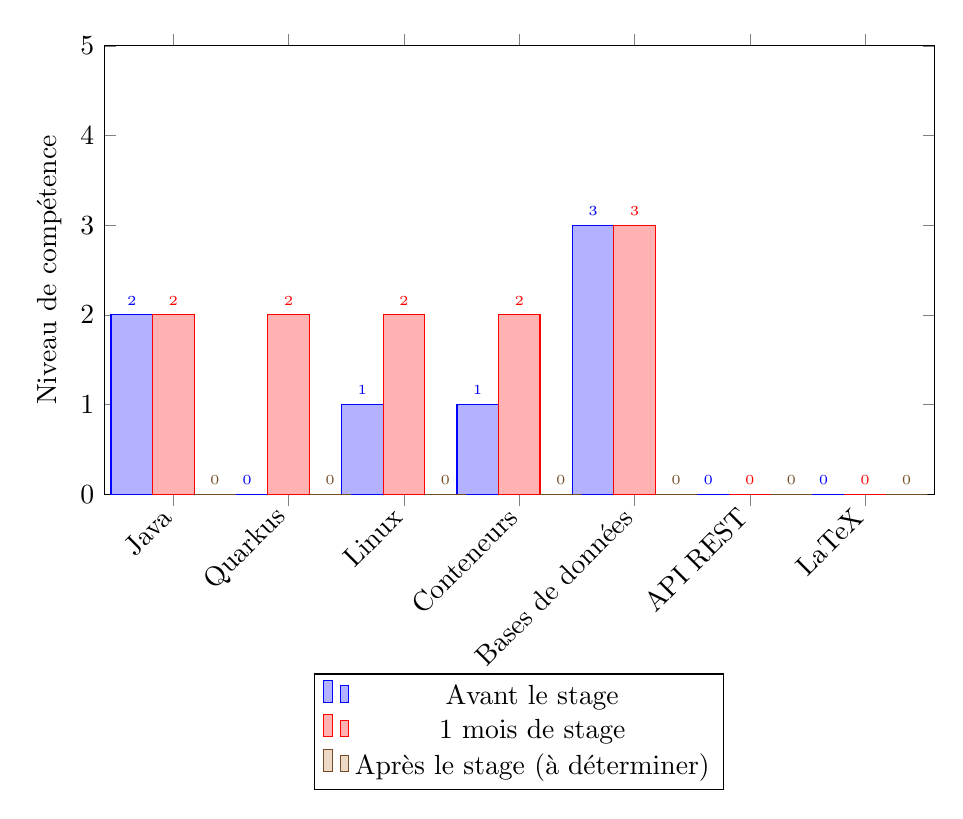
\begin{tikzpicture}
		\begin{axis}[
			ybar=0pt,
			bar width=15pt,
			symbolic x coords={Java, Quarkus,Linux, Conteneurs, Bases de données, API REST, LaTeX},
			xtick=data,
			x tick label style={rotate=45, anchor=east},
			ylabel={Niveau de compétence},
			xlabel={Compétences},
			legend style={at={(0.5,-0.4)}, anchor=north, legend columns=1}, % Légende beaucoup plus bas
			ymin=0,
			ymax=5,
			nodes near coords,
			every node near coord/.append style={font=\tiny},
			width=\textwidth,
			height=0.6\textwidth
			]
			% Données Avant le stage
			\addplot coordinates {(Java, 2) (Quarkus, 0) (Linux, 1) (Conteneurs, 1) (Bases de données, 3) (API REST, 0) (LaTeX, 0)};
			
			\addplot coordinates {(Java, 2) (Quarkus, 2) (Linux, 2) (Conteneurs, 2) (Bases de données, 3) (API REST, 0) (LaTeX, 0)};

			% Données Après le stage (à déterminer, on les met en blanc pour indication)
			\addplot coordinates {(Java, 0) (Quarkus, 0) (Linux, 0) (Conteneurs, 0) (Bases de données, 0) (API REST, 0) (LaTeX, 0)};
			
			\legend{Avant le stage,1 mois de stage, Après le stage (à déterminer)}
		\end{axis}
	\end{tikzpicture}
	
	\subsection{Efforts et résultats}
	
	à determiner
	
	\subsection{Ressenti personnel}
	
	à determiner
	
	\newpage
	\section{Bibliographie}
	\begin{itemize}
		\item \textbf{Documentation Quarkus} : Une ressource essentielle pour comprendre et utiliser Quarkus. Disponible sur : \url{https://quarkus.io/documentation/}
		\item \textbf{Documentation Flyway} : Guide pour utiliser Flyway dans Quarkus : \url{https://quarkus.io/guides/flyway}
		\item \textbf{Tutoriel sur HTTPie} : Introduction à l'utilisation de HTTPie pour tester des API REST. Disponible sur : \url{https://httpie.io/docs/cli}
		\item \textbf{Podman Documentation} : Documentation officielle pour apprendre à gérer des conteneurs avec Podman. Disponible sur : \url{https://podman.io/documentation}
		\item \textbf{Article sur OpenAPI et Redocly} : Tutoriel sur la génération de documentation statique avec OpenAPI et Redocly. Disponible sur : \url{https://redocly.com/docs/cli/} et demo : \url{https://dev.to/optnc/api-documentation-release-automation-with-github-redocly-and-open-api-f6h}
	\end{itemize}
	
\end{document}
